%!TEX program=xelatex
\documentclass[a4paper]{article}
%packages
\usepackage[UTF8]{ctex} %中文字符
\CTEXoptions[today=old]
\usepackage[left=2.50cm, right=2.50cm, top=2.50cm, bottom=2.50cm]{geometry} %调整页边距
\usepackage{xeCJK}
\usepackage{enumerate}%使用枚举
\usepackage{mathtools}
\usepackage{titlesec}
%\renewcommand{\thesection}{\chinese{section}.}%设置section
%\titleformat{\section}{\raggedright\large\rm\bf}{\thesection .\quad}{0pt}{}[]%右对齐4号字加粗标号后面有个点
\usepackage{bm}%加粗数学公式
\usepackage{amssymb}%因为所以
\usepackage{mathrsfs} %花体字
\usepackage{amsmath}%不太花的花体字
\usepackage[colorlinks,linkcolor=black,anchorcolor=blue,citecolor=green]{hyperref}%超链接
\renewcommand{\contentsname}{\centerline{目\ 录}}
\usepackage{indentfirst}%首行缩进
\setlength{\parindent}{2em}
\usepackage{graphicx}%图片
\usepackage{listings} %代码
\usepackage{xcolor}%颜色

\begin{document}
%%%%%%%%%%%%%%%%%%%%封面%%%%%%%%%%%%%%%%%%%%%
\title{接收机的设计与研究}
\author{ 施念 1120161302}
\maketitle{}
\newpage

%%%%%%%%%%%%%%%%%%%%%目录%%%%%%%%%%%%%%%%%%%%%
\begin{center}
\tableofcontents\label{c}
\end{center}
\newpage
%%%%%%%%%%%%%%%%%%%%正文%%%%%%%%%%%%%%%%%%%%%%
%%%%%%%%%%%%%%%%%%%%%%%%%%
\section{实验目的}
\begin{enumerate}[(1) ]
\item
掌握接收机的设计思路与设计方法,了解相关接收和匹配滤波的联系与区别。
\item
掌握Simulink的仿真方法,搭建接收机并对其进行分析与研究。
\item
探究不同调制方式对误码率的影响,结合理论分析实验结果。
\end{enumerate}

%%%%%%%%%%%%%%%%%%%%%%%%%%
\section{实验原理}
\subsection{最佳接收机}
\subsubsection{匹配滤波}
在线性输入(一般为确知信号叠加平稳噪声)的情况下,匹配滤波器是使\textbf{输出信噪比}达到最大的最佳滤波器,基于此可设计出最佳接收机。

匹配滤波器利用的频域特性(信号与噪声的频谱特性不同),采用的是频域分析法。当输入信号是简单的时域波形时,匹配滤波更容易实现($s(\tau-t)$)。匹配滤波器对于时延信号具有适应性,即对于时延信号来说,原信号的匹配滤波器仍能匹配滤波,只是最大峰值信噪比的发生时刻自动延迟$\tau$。
\subsubsection{相关接收}
相关接收从误码率最小的角度出发,得出最佳接收机的构成。相关接收分为自相关接收和互相关接收。自相关接收不需知道信号形式(参考信号中包含有噪声),收发信号一般不在同一地点;互相关接收需要知道信号形式,收发信号一般在同一地点。

互相关接收利用信号的时域特性(信号和噪声的相关时间不同),从时域进行分析。一般在输入信号是不确定的波形(如“噪声雷达”)时采用互相关接收。

\subsubsection{联系与区别}
对于互相关接收来说,输出$$Y(\tau)=\int_{-\infty}^{+\infty}X(t)s(t-\tau)dt=R_s(\tau)+R_{ns}(\tau)$$

当信号与噪声无关时$$Y(\tau)=\int_{-\infty}^{+\infty}X(t)s(t-\tau)dt=R_s(\tau)$$

此时互相关接收与匹配滤波是等效的。

匹配滤波可以用模拟方法实现,可以实时连续给出输出,但是相关接收只能在固定时延$\tau$时计算出互相关函数,若要得到全景图像,需要多次测量或者采用多路并联的方式。
%%%%%%%%%%%%%%%%%%%%%%%%%%
\section{实验内容}
\subsection{框图设计}
\subsubsection{总体框图}
在Simulink中,利用下图所示框图,对信号的发射、传输和接收过程进行仿真分析。
\begin{figure}[htbp]
\centering
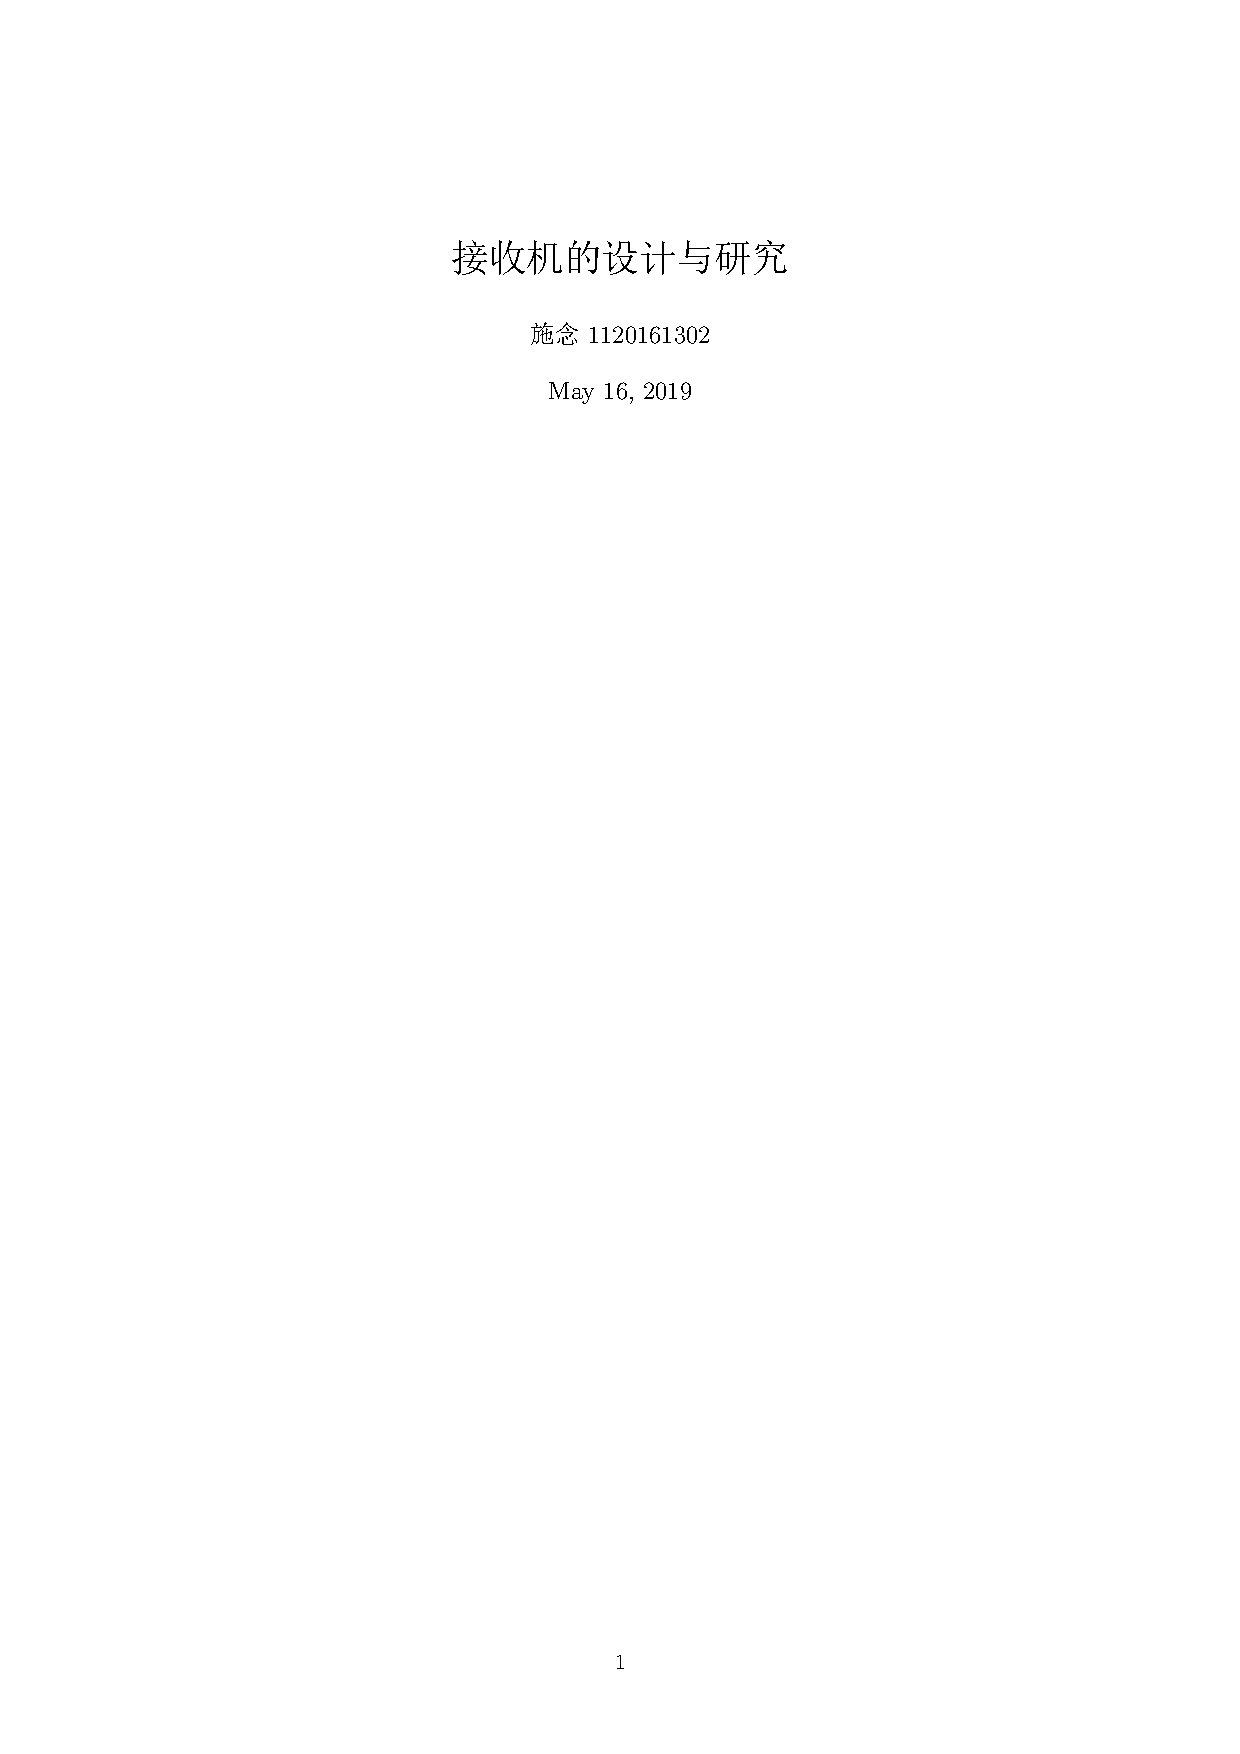
\includegraphics[scale=0.6]{imgs/receiver.png}
\caption{总体框图}
\end{figure}

如图所示,利用随机数发生器等概率的发送0和1,利用信号调制模块对信号进行调制,通过一个有噪信道到达接收端,在接收端进行利用相关接收对信号进行解调。最后通过误码率计算器对整个系统的误码率进行计算。

\subsubsection{BPSK部分}
系统中BPSK模块如下图所示
\begin{figure}[htbp]
\centering
\includegraphics[scale=0.6]{imgs/BPSK.png}
\caption{BPSK模块}
\end{figure}

在要发送1(>0)时,发送$s_{1}(t)=\sin(\omega t)$;要发送0时,发送$s_{0}(t)=-\sin(\omega t)$,即对信号进行BPSK调制。

\subsubsection{接收机部分}
系统中的主要部分——接收机部分如下图所示
\newpage

\begin{figure}[htbp]
\centering
\includegraphics[scale=0.6]{imgs/main.png}
\caption{接收机部分}
\end{figure}
 利用乘法器和积分器实现相关接收,即对于接收机输入端的信号,判断其与$s_1(t)$和$s_0(t)$的相关程度。积分复位利用一个脉冲信号实现,抽样判决利用“Zero-Order Hold”模块实现抽样功能,采用判决器模块判决功能(将抽样结果做差与门限进行比较),二者共同组成抽样判决器。需要注意的是,在积分器后要增加一个信号延迟,这样做的目的是为了使系统在很靠近最大积分输出处进行判决,避开积分复位使结果为1。

\subsection{系统仿真结果}
\subsubsection{原始信号、调制信号和接收信号}
用scope观察原始信号(0/1)、调制后的信号($s_1(t)$/$s_0(t)$)以及接收机的输入信号($s_t+n_t$),结果如下图所示,从图中可以看出,接收机的输入信号较为紊乱,因此必须要经过一定的判决方法才能实现对原信号的恢复。
\begin{figure}[htbp]
\centering
\includegraphics[scale=0.25]{receiver/receiver0.png}
\caption{a.原始信号 b.调制信号 c.接受信号}
\end{figure}

\subsubsection{接收机判决}
如下图所示,图a为抽样判决后的输出,图b为积分器输出,当$y_1(t) > y_0(t)$时,判为1,当$y_1(t) < y_0(t)$时,判为0。
\newpage
\begin{figure}[htbp]
\centering
\includegraphics[scale=0.4]{receiver/receiver1.png}
\caption{a.抽样判决输出 b.积分器输出}
\end{figure}

\subsubsection{输出信号对比}
将要发射的信号0/1和接收机的输出信号进行对比,如下图所示。图片中红色圆圈内为误判的错误情况。

\begin{figure}[htbp]
\centering
\includegraphics[scale=0.25]{receiver/receiver2.png}
\caption{a.发射信号 b.输出信号}
\end{figure}

需要注意的是,输出信号相对于输入信号有延时(1个单位/周期),在计算误码率时需要设置“delay”为1。分析可知,这是因为接收机在判决的时候需要进行积分操作(相当于匹配滤波器的延时)。

在仿真中,载波幅度为1,平均功率$S=0.5$,设置信噪比为-10dB。以此为前提下的误码率为$9\times 10^{-4}$。

\subsection{调制方式对$P_e$的影响}
\subsubsection{2FSK}
设计2FSK的结构框图如下图所示,通过一个switch模块对要发射的信号进行判断,当要发送1时,输出$\sin (\omega_1t)$,当要输出0时,输出$\sin (\omega_2t)$($\omega_2=2\omega_1$),判决门限为0。

\newpage

\begin{figure}[htbp]
\centering
\includegraphics[scale=0.35]{imgs/2FSK.png}
\caption{2FSK结构框图}
\end{figure}

仿真得到发送端输出以及接收机输入的信号波形如下图所示,在信噪比为-10dB的情况下,计算得到误码率为$1.35\times 10^{-2}$。

\begin{figure}[htbp]
\centering
\includegraphics[scale=0.25]{receiver/receiver4.png}
\caption{a.接收机输入 b.2FSK调制前后信号}
\end{figure}


\subsubsection{2ASK}
设计2ASK的结构框图如下图所示,总体结构与2FSK相似,不同的是,当要发送1时,输出$\sin (\omega t)$,当要输出0时,直接输出0。需要注意的是,如果要改变载波的幅度,门限也要随之改变。
\begin{figure}[htbp]
\centering
\includegraphics[scale=0.35]{imgs/2ASK.png}
\caption{2ASK结构框图}
\end{figure}
\newpage

仿真得到发送端输出以及接收机输入的信号波形如下图所示,在信噪比为3.98dB的情况下,计算得到误码率为$2.77\times 10^{-1}$。


\begin{figure}[htbp]
\centering
\includegraphics[scale=0.3]{receiver/receiver3.png}
\caption{a.接收机输入 b.2ASK调制前后信号}
\end{figure}


\subsubsection{总结与分析}
将上述实验结果进行整理,得到表1。分析下表可知,在信噪比相同的前提下,误码率BPSK<2FSK<2ASK。此题中2ASK采用的门限是a/2。虽然上面得出的结果符合理论知识,但是需要注意的是——这是在大信噪比情况下采用的逼近公式。

\begin{table}[h]
\centering
\caption{不同调制方式下的误码率对比}
\begin{tabular}[h]{ccc}
\hline
调制方式& 信噪比/SNR(dB)& 误码率($P_e$)\\
\hline
$2ASK$ &  -10 &$9\times 10^{-4}$\\
$2PSK$ &  -10 &$1.35\times 10^{-2}$\\
$2FSK$ &  -10 &$2.77\times 10^{-1}$\\
\hline
\end{tabular}
\end{table}

\subsection{信噪比对$P_e$的影响}
以信噪比为自变量,模拟不同污染程度的信道,利用BPSK对信号进行调制,利用相关接收对信号进行接收,分析接收处理后的信号的误码率,得到下图所示曲线。

\begin{figure}[htbp]
\centering
\includegraphics[scale=0.5]{imgs/PeSNR.png}
\caption{误码率随信噪比变化曲线}
\end{figure}

从仿真结果可以看出,随着信道信噪比的不断提升,误码率不断下降。在信噪比小于-10dB时,误码率升高速度加快;在信噪比小于-30dB时,接收机的接收判决效果已经很差,基本接近最坏的判决情况(即误码率$P_e=0.5$)。
% \subsection{多元信号接受机}



%%%%%%%%%%%%%%%%%%%%%%%%%%
\section{总结与分析}
\subsection{问题总结}
\begin{enumerate}[(1)]
\item
在simulink进行仿真时要注意时延对仿真结果的影响,如本实验中,因为要进行相关运算,所以在计算误码率时需要加一个单位的时延;在接收机部分,为了防止抽样判决时刻恰好和积分器的复位重合,需要在积分器后加一个很小的延时。
\item 
在进行仿真时,要注意门限对不同调制方式的影响。如在2ASK中,当改变信号幅度时,门限也要随之改变。并且需要注意的是,对于2ASK,其门限只有在信噪比较大的时候才能直接选取$a/2$。
\end{enumerate}

\subsection{实验总结}

在BPSK、2ASK、2FSK中,若采用相关接收,在BPSK对噪声的抵抗能力最强,2FSK次之,2ASK最差。相对于2ASK,2PSK对信道特性不敏感,判决门限不会随着信道改变而改变。BPSK用相位来传递信息,但是在实际过程中会有一定的相位模糊,因此会采用2DPSK。相对于2FSK,2PSK更容易实现,并且2PSK对频谱利用率更高。在实际应用中,为了提高传输效率,一般会牺牲一部分的误码率,采用MPSK(如QPSK)。


\end{document}}